\documentclass[11pt]{article}
\usepackage{amsmath}
\usepackage{tikz}
\usepackage[left=3cm, right=3cm, top=3cm, bottom=3cm]{geometry}
\setlength{\parindent}{0pt} % Remove paragraph indent
% \pagestyle{empty} % Remove page numbers

\title{COMP4621 Programming Assignment}
\date{\today}
\author{TSOI Chun Wong (20956530)}
\begin{document}
\maketitle

\section{Overview}

This programming assignment implements a chat room system with 
one TCP server, multiple TCP clients, and UDP peer-to-peer messaging. \\

Main features: 
\begin{itemize}
    \item Server handles multiple clients with \texttt{poll()} and manages user information state and message broadcasting.
    \item Clients use threads to send commands and receive messages concurrently from the server and peers.
    \item Peer-to-peer direct messaging over UDP with a reliable data transfer protocol (RDT 3.0).
\end{itemize}

Other features include registration and login, user directory lookup, and offline message storage.

\section{Design}

\subsection{Server}

The server uses \texttt{poll()} to handle multiple connected clients in one process. 
It keeps a list of registered users and tracks each of their usernames, 
IP addresses, ports, and online/offline status. 
This is required so that it can redirect and broadcast any public messages, 
as well as answer \texttt{DIR} requests from clients and store offline messages for later delivery.

\subsection{Client}
The client uses \texttt{pthreads} so that it can accept constant real-time input from the terminal 
while receiving messages from both the server and other clients. 
TCP is used for communication with the server, while UDP is used for peer-to-peer direct messages. 
For UDP reliability, we use a simple style RDT 3.0 protocol with sequence numbers, 
ACK messages, retries (10 maximum), and timeouts.

\section{Implementation}

\subsection{Registration and Login}
When a new client connects to the server, it must first register with a unique username. 
The server checks if the username is already taken and responds accordingly. 
This requires the client creating a TCP socket and connecting to the server, 
where the server will then accept this connection and 
add the new file descriptor (the client) to its list of users managed by \texttt{poll()}., 
as well as requesting the client to send its username. \\

Upon successful TCP connection, the client is now successfully registered and logged in.
the client will receive a welcome message from the server and the menu display.
The server will also announce the new user's arrival to all other online clients.

\subsection{Client-server Communication}
Once registered / logged in, the client can send messages and commands to the server. 
Messages will be re-broadcasted to all other online clients, 
while commands like \texttt{DIR} will trigger a server response with the requested information.
These communications are done solely through the TCP connection established during login. \\

On the receiving side, the client has a background thread that listens for incoming messages from the server. 
We will call it the "server listener thread". 
A mutex is used to protect shared access to flags and buffers between several client threads.
A conditional variable is added to help avoid busy-waiting for certain flags and server responses.
After acquiring the mutex, the server listener thread can then process the received message, print it, 
and update any relevant states (more details below) 
if the message was a response to a client \texttt{DIR} request or an offline message delivery. 

\subsection{\texttt{DIR} Command}
The server keeps track of all registered users, 
their online/offline status, and their IP and port information.
The server receives updates when clients register or log in, as well as when they disconnect. \\

When the client inputs a \texttt{DIR} command to the server, 
the server returns a response containing the list of all registered users, 
their online/offline status, and their IP and port information. 
The client's server listener thread will then parse this response, 
update the conditional variable to unblock the main thread, 
and pass the user information into a shared buffer for the main thread to read.
Only the usernames and online statuses are displayed.

\subsection{Peer-to-peer Messaging}
For direct messaging, the client first need to obtain the information of the recipient. 
This can be attained by sending a \texttt{DIR} request to the server, 
receiving the full list of users and their IP/port information, 
and then searching for the intended recipient among the results. \\

If the recipient is offline, the sender client will send the offline message to the server, 
which will be redirected to the recipient when they next log in. 
See the next subsection for details on offline message storage and delivery. \\

If the recipient is online, UDP will then be used to send the message directly to the recipient. 
Clients, during launch, initiate a background thread that listens for incoming UDP messages.
We will call it the "peer listener thread". 
The sender client will create a UDP socket and send the message to the recipient's IP and port. 
The RDT 3.0 protocol splits long messages into chunks, 
then sends each chunk with a sequence number and waits for the correct ACK with a timeout before moving on. 
The receiver's peer listener thread reassembles the chunks and 
prints the full message only after the last fragment arrives. \\

If the sender keeps timing out and does not receive the correct ACK after 10 retries, 
the receipient is deemed unreachable and the client will fallback to offline message delivery.

\subsection{Offline Message Storage and Delivery}
When a client wishes to send a direct message to an offline recipient,
the sender client will instead send the message to the server (over TCP), 
which will then be stored in a list of pending messages in the format of a txt file.
This format allows the server to persist messages even if it restarts, 
and also avoids strict memory allocation constraints for pending messages for the same recipient. \\

When the recipient next logs in, 
the server will check if there are any pending messages for them and deliver them (over TCP).
The client's server listener thread will then update the conditional variable to unblock the main thread, 
and pass the pending messages into a shared buffer for the main thread to read, process and print.

\subsection{Exit and Logout}
When a client inputs the \texttt{EXIT} command, 
the client will first send a logout message to the server, updating the user's status to offline, 
at the same time removing the client's file descriptor from the \texttt{poll()} list.
The client will then close its TCP and UDP sockets and exit the program.
The server will also update the user's status to offline if it detects that 
the client has disconnected without sending a logout message. 
The server will announce the user's departure from the chat room to all other online clients.

\section{Testing}
Program passes all tests in the provided \texttt{grader\_linux.sh} test script, 
which includes registration, login, message broadcasting, \texttt{DIR} command, 
peer-to-peer messaging, rdt 3.0 recovery, offline message delivery, and exit/logout. \\

System behavior has also been manually tested and verified within an Ubuntu Linux environment, 
since Windows environment does not provide the full POSIX socket and threading library required.

\section{BONUS: Simple GUI using ncurses}
A simple text-based GUI is implemented using the \texttt{ncurses} library, 
dividing the terminal into three panes: 
a friends list on the left, a large message display in the middle, and an input area at the bottom. \\

See the screenshot below for an example of the GUI in action:

\begin{center}
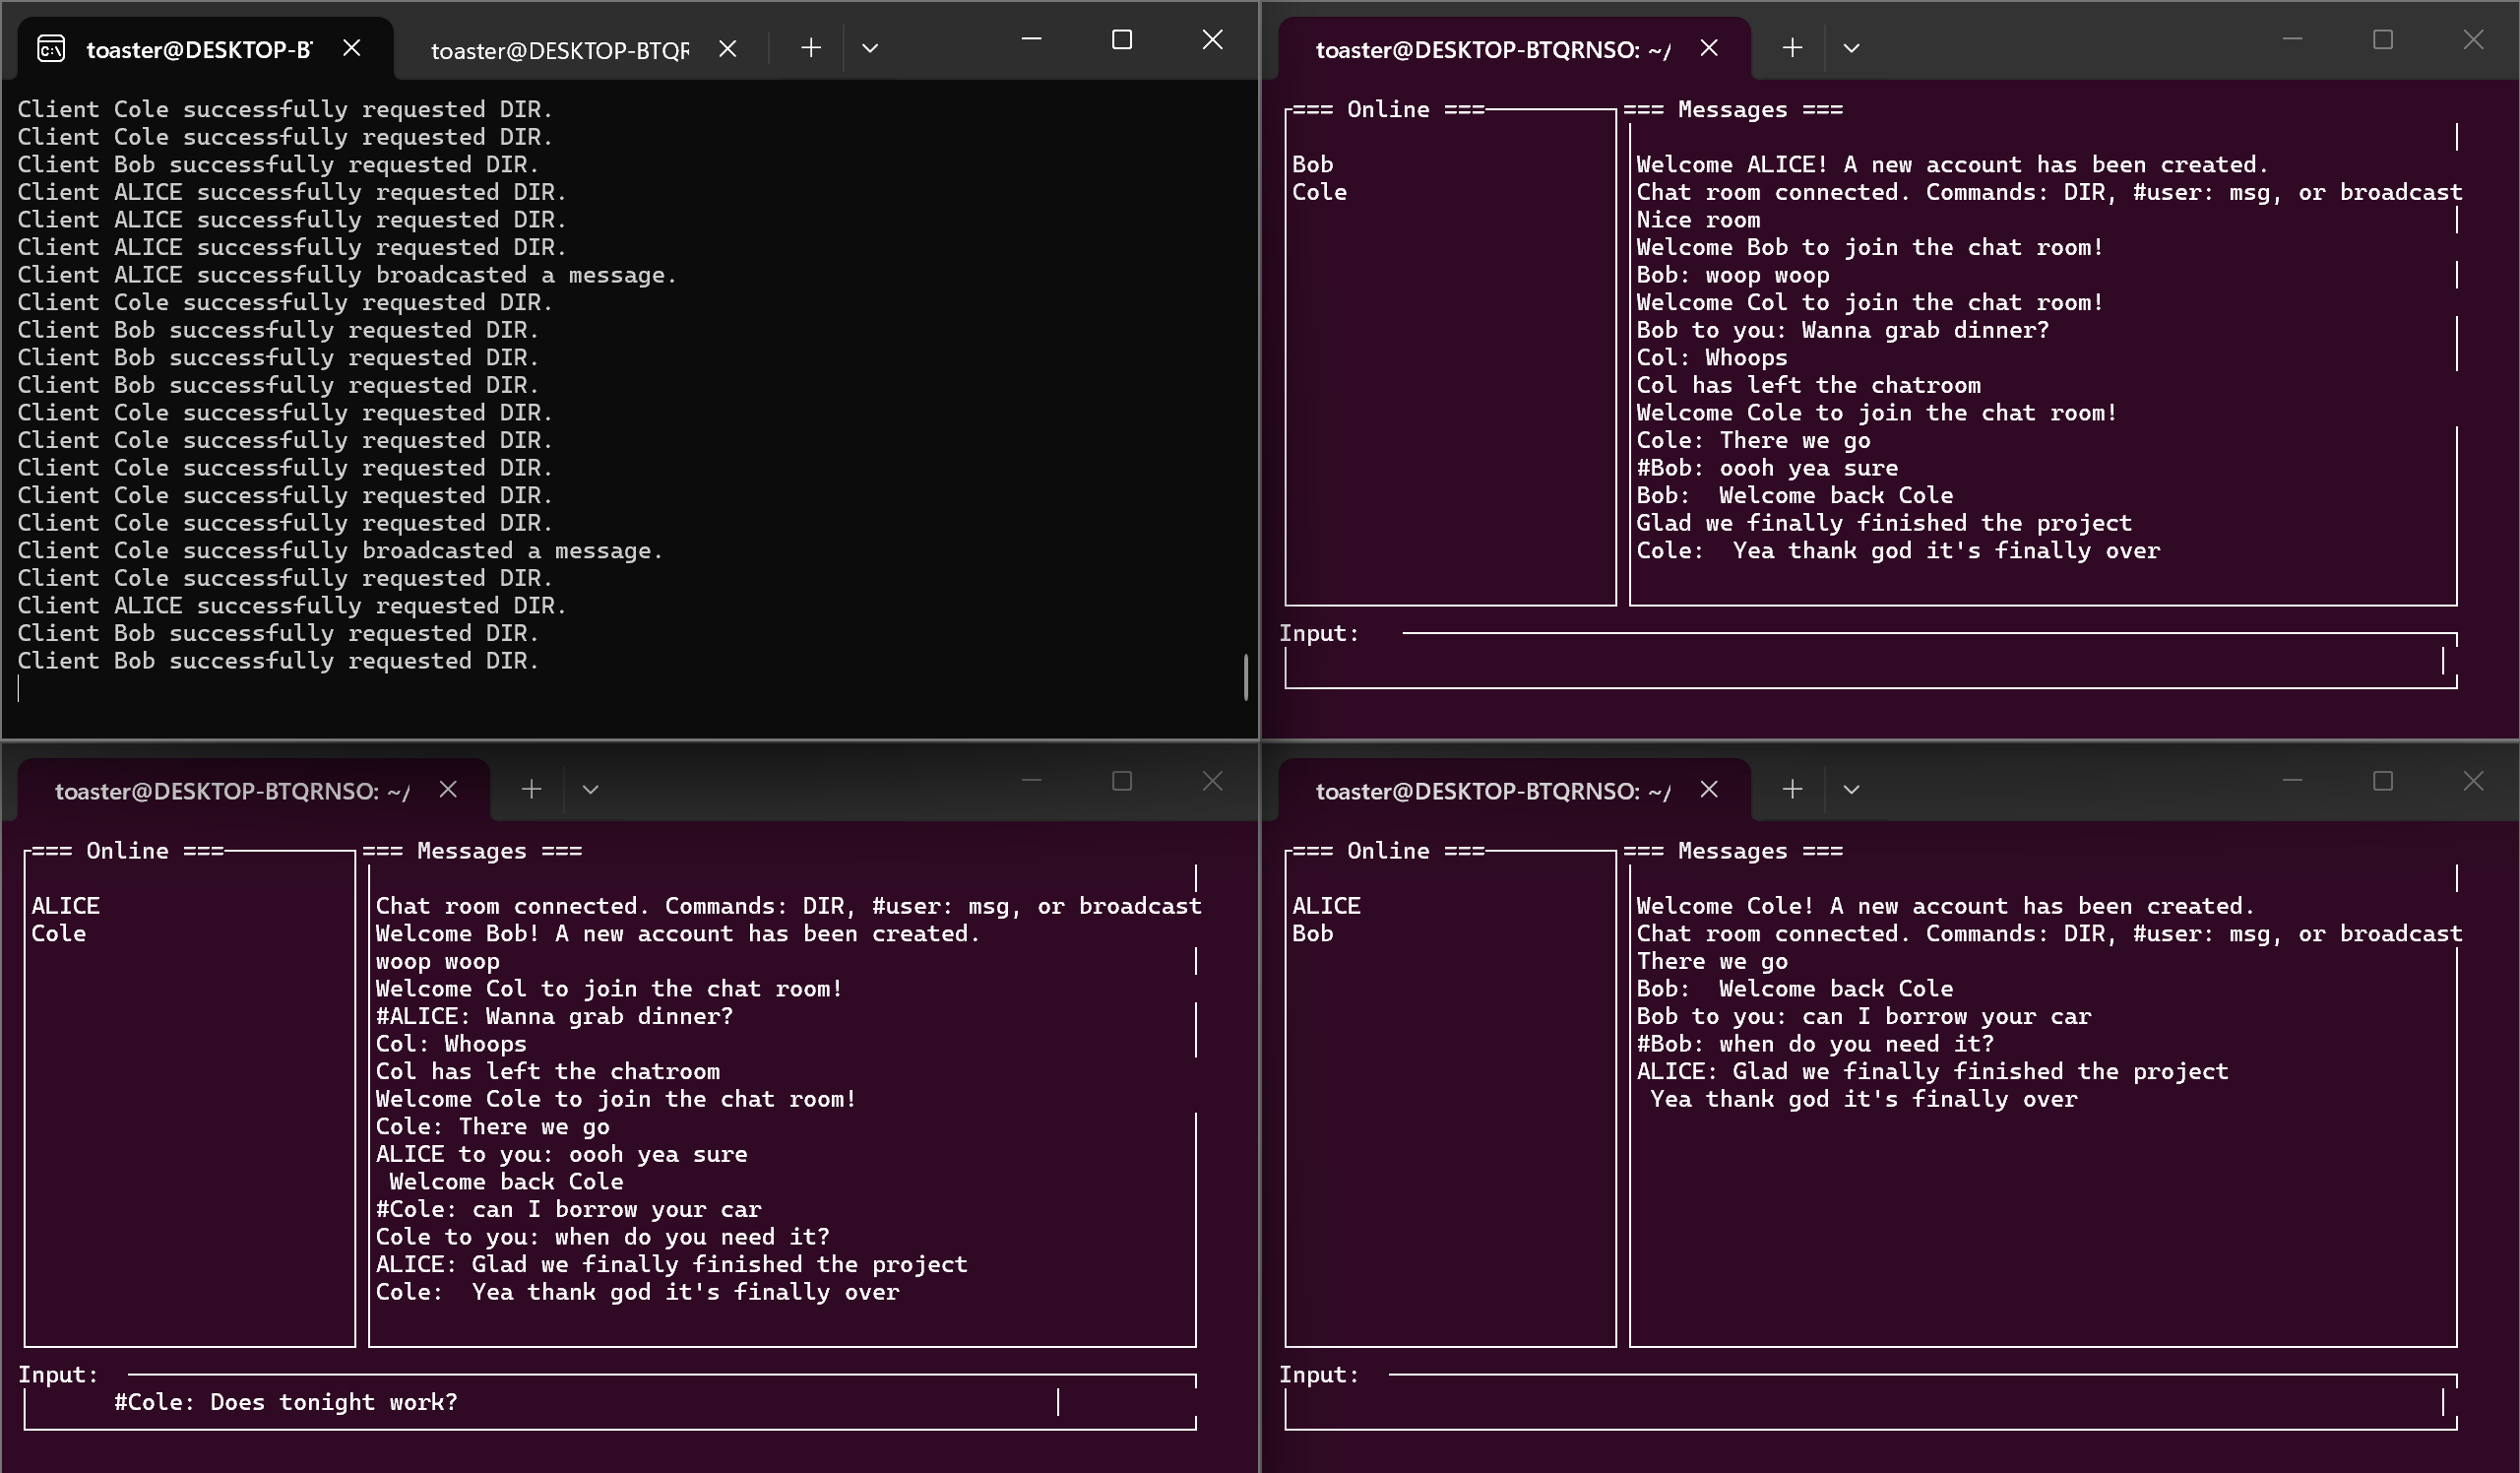
\includegraphics[width=0.8\textwidth]{gui_screenshot.png}
\end{center}

The screenshot shows 3 clients connected to the server, with the top left pane displaying server logs. \\

An unsolved issue with the GUI is that they do not refresh automatically. 
Currently, the GUI updates only when the window detects user input in the form of keystrokes, 
leading to desynced UI and messages until the user interacts with the terminal.
However, the basic functionality of the chat system is unaffected by this issue, 
and the GUI still serves as a decent visual aid 
for users to view messages and online users in a more organized manner.

\section{Conclusion}

The final result is a chat room system that supports server-based coordination, 
peer-to-peer messaging, offline fallback, and basic reliability over UDP. 


\end{document}